\section{Results} \label{sec:results}

We employ the optimization described above (see \equref{eq:opt}) in an interactive freeform editing system. The input to our system is the flat domain boundary and the curves of the crease pattern, represented by polylines. These can be easily generated from any standard vector graphics format by sampling the smooth curves therein. Our system computes an arrangement of the input curves using CGAL's arrangement model \cite{cgal,cgal_arr1,cgal_arr2} and solves the symmetric indefinite  linear systems as required by the optimization (\equref{eq:linear_system}) using Pardiso \cite{PARDISO1,PARDISO2,PARDISO3}. \newt{We ran our experiments on a 16-core Ryzen Threadripper 1950X clocked at \unit[3.4]{GHz}}. Our editing system supports setting point handle positional constraints, as can be seen in Figures \ref{fig:teaser}, \ref{fig:multiple_crease_patterns}, \ref{fig:ring}, and the second and last model from the left in \figref{fig:folded_and_not_folded}. A stress test for our algorithm is shown in \figref{fig:ring}, with a crease pattern containing $20$ different creases that all automatically bend and fold, driven only by point handle positional constraints. We also support  constraining a crease curve by specifying its curvature and torsion in a curve constrained flow,  see Figures~\ref{fig:folded_and_not_folded} and \ref{fig:MV_bias_modeling}, as well as prescribing a sparse set of dihedral angles along crease points, see \figref{fig:dihedral_editing}. 

\figref{fig:MV_bias_modeling} is the only case where we supply a mountain/valley assignment as input, while \figref{fig:dihedral_editing} displays the only models designed by constraining dihedral angles. The curve constrained positional constraints, as well as the dihedral angles, are interpolated for improved quality (see \figref{fig:homotopy_curve}). To maintain interactive frame rates in handle based editing tasks, we run a fixed number of SQP iterations per frame, which we set to 5. \newt{On models with 500, 1000, 2000, 4000 vertices these 5 SQP iterations run on average at more than 39, 19, 9, 4 frames per second.} Hence our system is able to handle realtime interaction of meshes with around 2000 vertices. The two concentric circles folds in \figref{fig:teaser} originate from a mesh with about 5500 vertices. They are designed by simply penalizing the distance of a single pair of vertices while interpolating the penalty weight, and their final forms are reached in about 30 seconds. We refer the reader to our supplementary video for further results, including interactive editing examples. 

\begin{figure} [t]
	\centering
	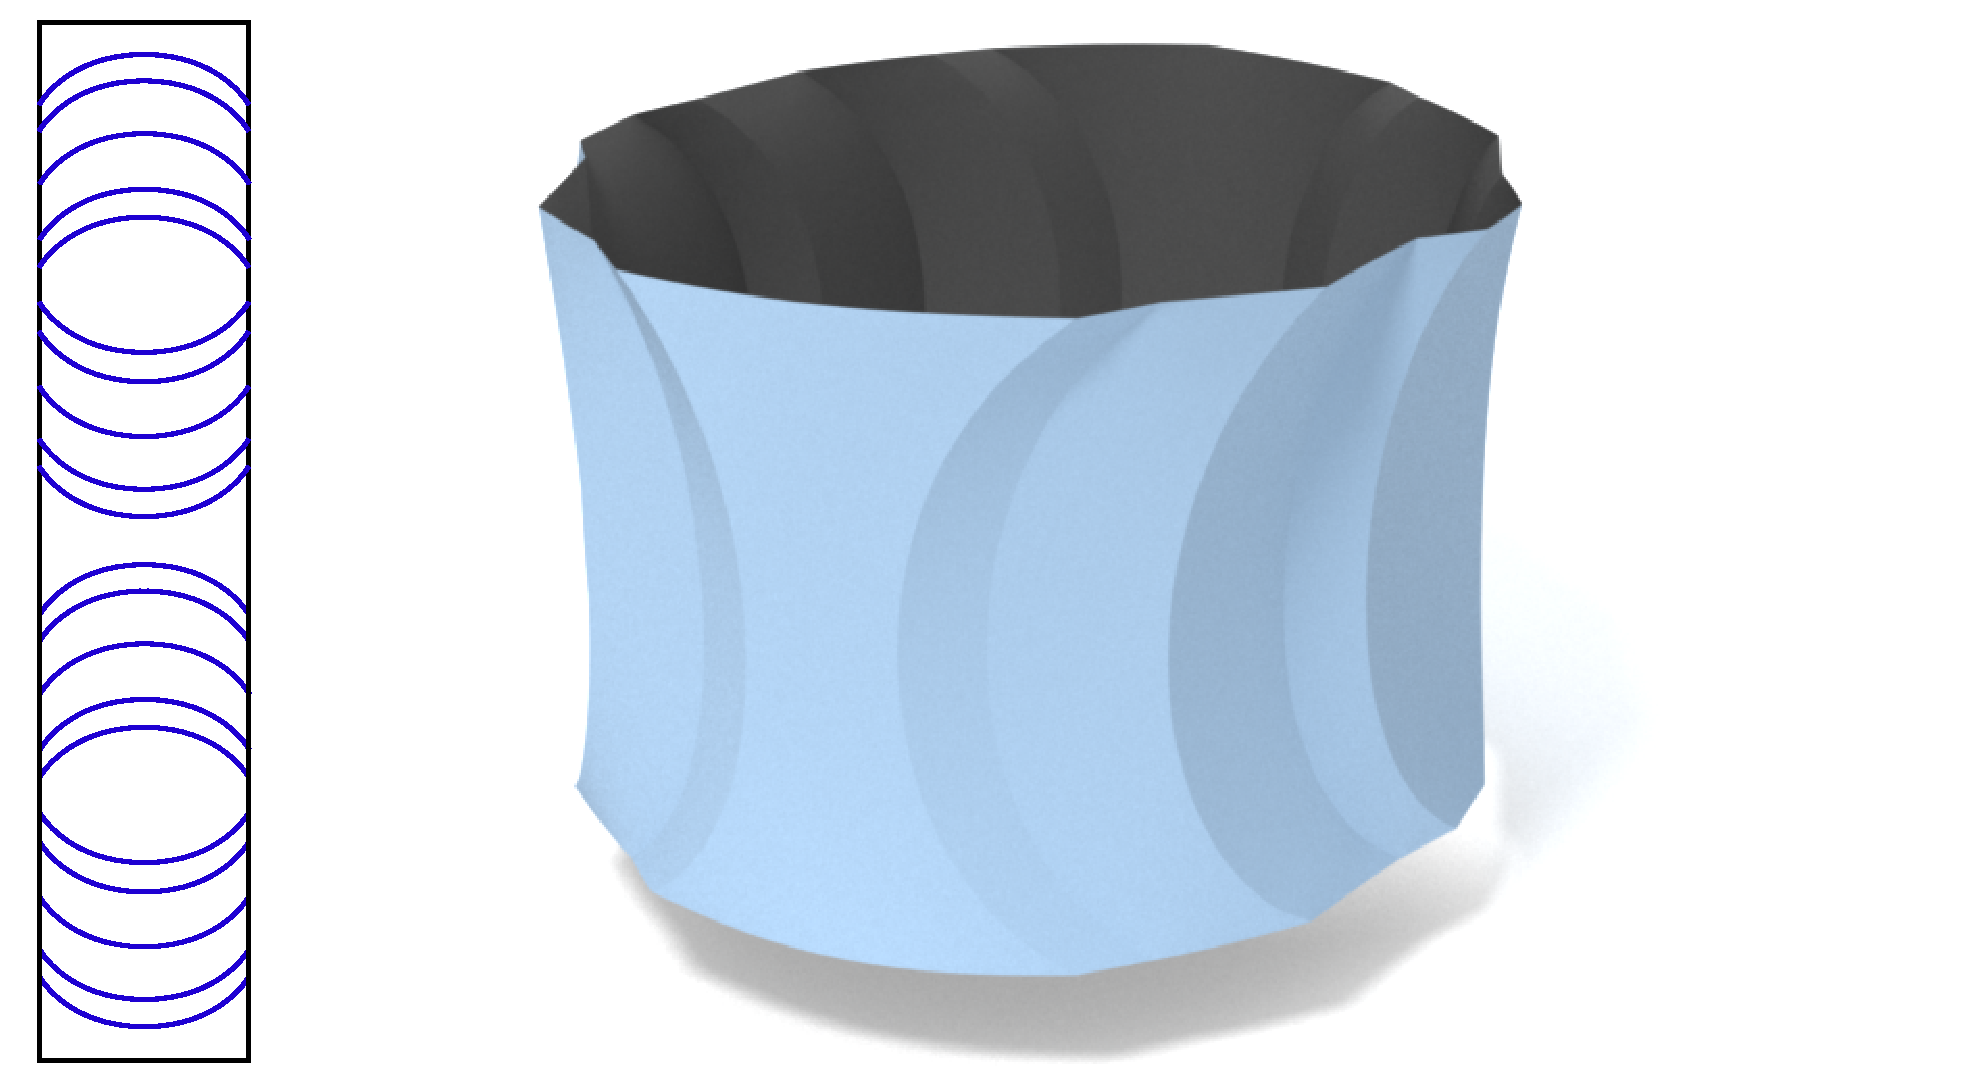
\includegraphics[width=0.65\linewidth]{figures/ring}
	\caption{A curved folded ring. The crease pattern is taken from \cite{mitani2019curved} and contains 20 different creases. \newt{It was deformed by enforcing our folding constraints (\secref{sec:implementation}), without specifying any folding angles or mountain/valley assignments}, together with positional constraints pushing the vertices on the right and left boundary to match such that a loop is formed, while also minimizing an additional bending energy term for the glued area to smooth it.}
	\label{fig:ring}
\end{figure}